\documentclass[11pt,a4paper]{article}
\usepackage[margin=1in]{geometry}
\usepackage[T1]{fontenc}
\usepackage[utf8]{inputenc}
\usepackage{graphicx}
\usepackage{booktabs}
\usepackage{float}
\usepackage{tabularx}
\usepackage{array}
\usepackage{hyperref}
\usepackage{xcolor}
\hypersetup{colorlinks=true,linkcolor=blue,urlcolor=blue}

\title{SEM Dendrite Segmentation: Comparative Technical Report}
\author{Automated Report Generator}
\date{\today}

\begin{document}
\maketitle

\section*{Abstract}
This report summarizes pixel-level semantic segmentation of lithium dendrites in SEM images using two pipelines:
(1) a deterministic classic morphology pipeline and
(2) a YOLO segmentation model.
The evaluation set includes 14 labeled images.
Average Dice scores are Classic=0.845 and YOLO=0.449.
The report includes quantitative metrics, method comparison tables, and visual success/failure analysis.

\section*{Methodology}
\subsection*{Classic Pipeline (\texttt{scripts/classic\_scripts/classic\_pipeline.py})}
The classical pipeline is deterministic and is executed in fixed stages:
\begin{enumerate}
\item \textbf{Input and cleanup:}
each SEM image is loaded in grayscale, then the bottom instrument region (scale bar / metadata strip) is removed using \texttt{remove\_scale\_bar}.

\item \textbf{Pre-processing (\texttt{preprocess}):}
\begin{itemize}
\item \texttt{normalize\_histogram}: linear stretch to full \([0,255]\), reducing exposure variation across images.
\item \texttt{apply\_clahe}: local contrast enhancement for weak dendrite visibility.
\item \texttt{apply\_bilateral\_filter}: denoising while preserving thin branch edges.
\end{itemize}

\item \textbf{Segmentation (\texttt{segment\_adaptive}):}
adaptive Gaussian thresholding is applied with local neighborhood size \texttt{ADAPTIVE\_BLOCK\_SIZE} and bias \texttt{ADAPTIVE\_C}. This is preferred over global thresholding due to non-uniform illumination in SEM images.

\item \textbf{Post-processing (\texttt{postprocess}):}
\begin{itemize}
\item \texttt{morphological\_reconstruction}: geodesic reconstruction after erosion to suppress noise while preserving dendrite geometry.
\item \texttt{apply\_closing}: fills small holes and improves branch continuity.
\item \texttt{remove\_small\_components} (enabled by profile): removes isolated small blobs unless proximity logic indicates likely branch continuation.
\end{itemize}

\item \textbf{Branch separation (\texttt{separate\_branches}):}
distance transform + marker-based watershed separates touching dendrites by cutting watershed boundaries.

\item \textbf{Skeletonization and outputs:}
\texttt{skeletonize\_mask} extracts a 1-pixel centerline from the final mask. Masks/skeletons are restored to the original canvas size, and intermediate artifacts are saved (\texttt{01\_original} ... \texttt{12\_preview}) for traceability.
\end{enumerate}

\subsubsection*{Classic Parameter Profiles Used in This Project}
The orchestrator (\texttt{scripts/run\_all.py}) applies profile-specific parameters by subset (\texttt{dataset/easy} vs \texttt{dataset/hard}) through \texttt{apply\_parameter\_profile}.

\textbf{Common baseline parameters (shared unless overridden):}
\texttt{CLAHE\_CLIP\_LIMIT}=1.0,
\texttt{CLAHE\_TILE\_SIZE}=8,
\texttt{BILATERAL\_D}=9,
\texttt{BILATERAL\_SIGMA\_COLOR}=50,
\texttt{BILATERAL\_SIGMA\_SPACE}=50,
\texttt{ADAPTIVE\_BLOCK\_SIZE}=67,
\texttt{ADAPTIVE\_C}=-12,
\texttt{EROSION\_KERNEL\_SIZE}=5,
\texttt{EROSION\_ITERATIONS}=1,
\texttt{CLOSING\_KERNEL\_SIZE}=3,
\texttt{DISTANCE\_THRESHOLD}=0.07,
\texttt{COMPONENT\_PROXIMITY\_RADIUS}=30,
\texttt{COMPONENT\_PROXIMITY\_RATIO}=0.5.

\textbf{Easy profile (\texttt{dataset/easy}) overrides:}
\texttt{RUN\_SMALL\_REMOVAL}=True,
\texttt{MIN\_COMPONENT\_AREA}=75.

\textbf{Hard profile (\texttt{dataset/hard}) overrides:}
\texttt{RUN\_SMALL\_REMOVAL}=True,
\texttt{MIN\_COMPONENT\_AREA}=450,
\texttt{COMPONENT\_PROXIMITY\_RADIUS}=50.

\subsection*{Deep Learning Pipeline (\texttt{scripts/yolo\_scripts/yolo\_pipeline.py})}
The deep model is Ultralytics YOLO segmentation (\texttt{yolo11x-seg.pt}) with transfer learning.
\begin{enumerate}
\item \textbf{Dataset normalization:}
\texttt{ensure\_three\_channel\_dataset} converts grayscale / single-channel / BGRA images to 3-channel BGR PNG and clears stale cache files, ensuring compatibility with pretrained YOLO backbones.

\item \textbf{Training setup used:}
from the saved run arguments (\texttt{output/yolo/train/dendrite\_seg/args.yaml}): model=\texttt{yolo11x-seg.pt}, epochs=100, image size=640, batch=8, initial learning rate \(lr0=0.001\), patience=0, freeze=0, workers=0.

\item \textbf{Inference and mask extraction:}
inputs are normalized by \texttt{\_prepare\_image\_for\_yolo} (channel fix + dtype normalization), then \texttt{predict\_batch} runs inference with confidence threshold \texttt{conf}=0.25. All instance masks are resized to image resolution and merged with logical OR (\(mask > 0.5\)) to produce a final binary \(\{0,255\}\) mask per image.
\end{enumerate}

\subsection*{Evaluation Metrics}
Both pipelines are evaluated against manual ground truth using Dice, IoU, Precision, and Recall. Failure analysis is then derived from metric patterns (over-segmentation vs under-segmentation vs fundamental mismatch).

\section*{Results and Discussion}
The discussion below focuses on operational behavior: stability, typical error modes, and deployment implications.

\subsection*{Average Metrics}
\begin{table}[H]
\centering
\begin{tabular}{lcccc}
\toprule
Method & Dice & IoU & Precision & Recall \\
\midrule
Classic & 0.845 & 0.787 & 0.788 & 0.932 \\
YOLO & 0.449 & 0.302 & 0.335 & 0.709 \\
\bottomrule
\end{tabular}
\caption{Average segmentation metrics across available predictions.}
\end{table}
Classic clearly outperforms YOLO in this run (Dice 0.845 vs 0.449 and IoU 0.787 vs 0.302), indicating better overlap quality with manual masks.
Classic recall is also consistently high, while YOLO shows weaker precision and lower overlap consistency, reflecting frequent over-segmentation or domain mismatch.

\subsection*{Per-Image Comparison}
\begin{table}[H]
\centering
\scriptsize
\begin{tabular}{lcccccccc}
\toprule
Image & C-Dice & C-IoU & C-Prec & C-Rec & Y-Dice & Y-IoU & Y-Prec & Y-Rec \\
\midrule
2e-9\_100s\_002 & 0.923 & 0.857 & 0.857 & 1.000 & 0.579 & 0.407 & 0.409 & 0.991 \\

2e-9\_100s\_014 & 0.931 & 0.872 & 0.872 & 1.000 & 0.655 & 0.487 & 0.560 & 0.789 \\

2e-9\_100s\_017 & 0.699 & 0.538 & 0.538 & 1.000 & 0.103 & 0.055 & 0.066 & 0.241 \\

2e-9\_100s\_019 & 0.997 & 0.995 & 0.995 & 1.000 & 0.596 & 0.424 & 0.454 & 0.865 \\

70nm\_diameter\_100nm\_pitch\_008 & 0.927 & 0.863 & 0.863 & 1.000 & 0.438 & 0.280 & 0.302 & 0.798 \\

70nm\_diameter\_100nm\_pitch\_012 & 0.919 & 0.850 & 0.850 & 1.000 & 0.523 & 0.354 & 0.399 & 0.758 \\

70nm\_diameter\_100nm\_pitch\_022 & 0.995 & 0.991 & 0.991 & 1.000 & 0.454 & 0.293 & 0.374 & 0.577 \\

70nm\_diameter\_100nm\_pitch\_031 & 1.000 & 1.000 & 1.000 & 1.000 & 0.359 & 0.218 & 0.272 & 0.527 \\

70nm\_diameter\_100nm\_pitch\_033 & 0.024 & 0.012 & 0.017 & 0.043 & 0.065 & 0.034 & 0.039 & 0.194 \\

Ag\_1e-8\_008 & 1.000 & 1.000 & 1.000 & 1.000 & 0.436 & 0.278 & 0.325 & 0.660 \\

Ag\_1e-9\_\_02\_016 & 0.906 & 0.828 & 0.828 & 1.000 & 0.560 & 0.389 & 0.432 & 0.796 \\

Ag\_2e-9\_013 & 0.760 & 0.612 & 0.612 & 1.000 & 0.518 & 0.350 & 0.351 & 0.994 \\

Ag\_2e-9\_014 & 0.753 & 0.603 & 0.603 & 1.000 & 0.479 & 0.315 & 0.316 & 0.994 \\

Ag\_40nm\_pitch\_014 & 1.000 & 1.000 & 1.000 & 1.000 & 0.514 & 0.346 & 0.395 & 0.736 \\
\bottomrule
\end{tabular}
\caption{Per-image metric comparison (first 14 rows). Full table is exported to CSV.}
\end{table}
The per-image table shows that Classic remains strong on most samples, including several near-perfect cases (Dice close to 1.0).
YOLO performance is more variable: moderate on some images but significantly degraded on others, especially where texture statistics differ from the training distribution.
The most severe outlier (\texttt{70nm\_diameter\_100nm\_pitch\_033}) affects both methods and should be treated as a hard-failure sample in downstream workflows.

\subsection*{Failure Analysis}
Number of failures under Dice threshold: 8.
\begin{table}[H]
\centering
\scriptsize
\begin{tabularx}{\linewidth}{llcccX}
\toprule
Image & Method & Dice & Precision & Recall & Estimated Cause \\
\midrule
70nm\_diameter\_100nm\_pitch\_033 & Classic & 0.024 & 0.017 & 0.043 & Fundamental mismatch - wrong region or severe artifacts \\

70nm\_diameter\_100nm\_pitch\_033 & YOLO & 0.065 & 0.039 & 0.194 & Fundamental mismatch - wrong region or severe artifacts \\

2e-9\_100s\_017 & YOLO & 0.103 & 0.066 & 0.241 & Fundamental mismatch - wrong region or severe artifacts (Classic succeeds -> likely OOD sample for YOLO) \\

70nm\_diameter\_100nm\_pitch\_031 & YOLO & 0.359 & 0.272 & 0.527 & Fundamental mismatch - wrong region or severe artifacts (Classic succeeds -> likely OOD sample for YOLO) \\

Ag\_1e-8\_008 & YOLO & 0.436 & 0.325 & 0.660 & Over-segmentation - noise included as dendrite (Classic succeeds -> likely OOD sample for YOLO) \\

70nm\_diameter\_100nm\_pitch\_008 & YOLO & 0.438 & 0.302 & 0.798 & Over-segmentation - noise included as dendrite (Classic succeeds -> likely OOD sample for YOLO) \\

70nm\_diameter\_100nm\_pitch\_022 & YOLO & 0.454 & 0.374 & 0.577 & Fundamental mismatch - wrong region or severe artifacts (Classic succeeds -> likely OOD sample for YOLO) \\

Ag\_2e-9\_014 & YOLO & 0.479 & 0.316 & 0.994 & Over-segmentation - noise included as dendrite (Classic succeeds -> likely OOD sample for YOLO) \\
\bottomrule
\end{tabularx}
\caption{Failure characterization based on precision/recall patterns.}
\end{table}
Failure patterns are asymmetric between methods.
Most flagged YOLO failures combine low precision with moderate-to-high recall, which matches over-segmentation (false-positive expansion into background structures).
Classic has one major failure on the same outlier image, suggesting a true data difficulty case rather than a single-model artifact.
From a risk perspective, this supports Classic as baseline and YOLO as auxiliary signal rather than primary mask source in the current configuration.

\subsection*{Visual Analysis (Successes and Failures)}
\begin{figure}[H]
\centering

\includegraphics[width=0.96\linewidth]{assets/cases/70nm_diameter_100nm_pitch_022_analysis.png}
\caption{Success case: 70nm\_diameter\_100nm\_pitch\_022 (combined Dice=0.670)}
\end{figure}

\begin{figure}[H]
\centering
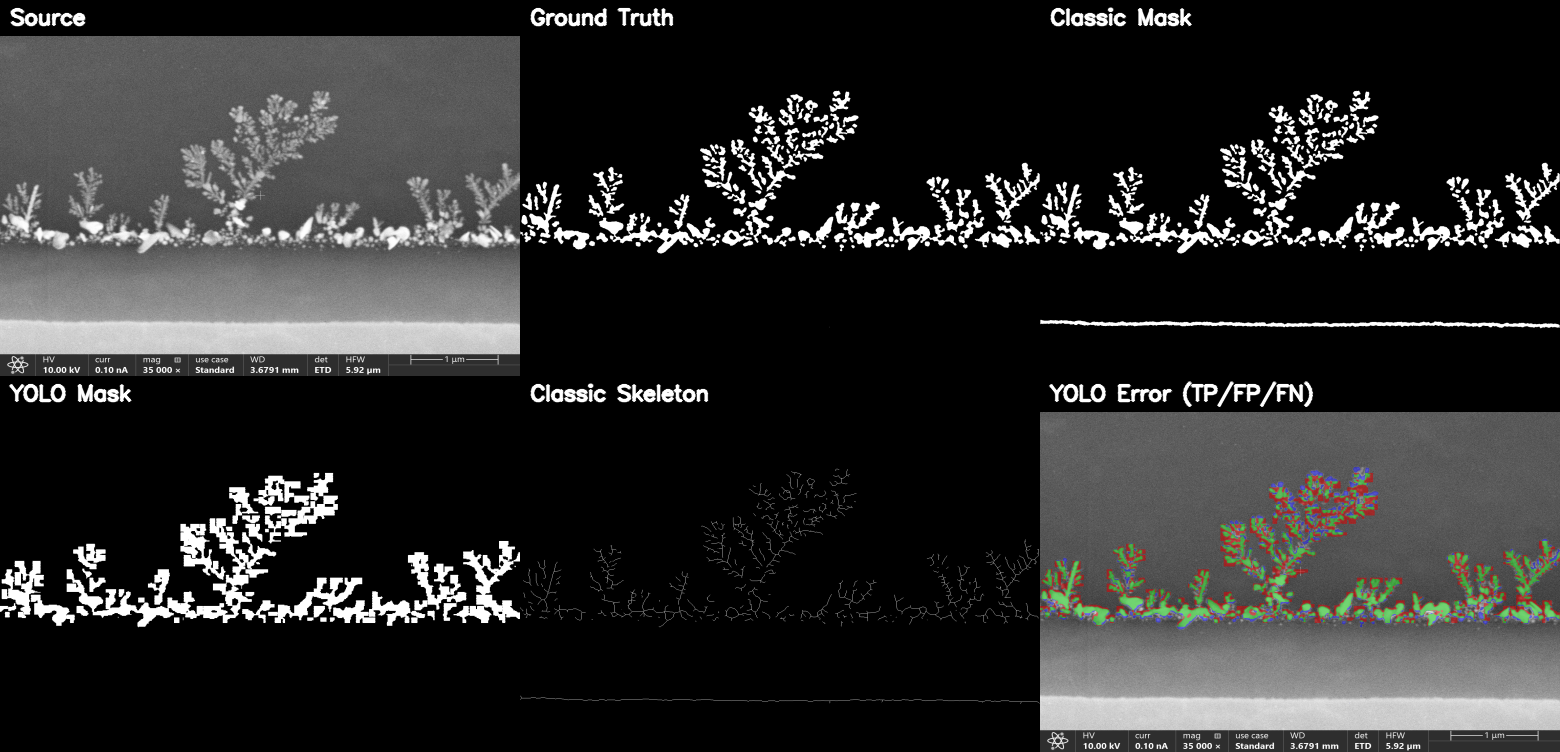
\includegraphics[width=0.96\linewidth]{assets/cases/2e-9_100s_014_analysis.png}
\caption{Success case: 2e-9\_100s\_014 (combined Dice=0.465)}
\end{figure}

\begin{figure}[H]
\centering

\includegraphics[width=0.96\linewidth]{assets/cases/70nm_diameter_100nm_pitch_033_analysis.png}
\caption{Failure case: 70nm\_diameter\_100nm\_pitch\_033 (combined Dice=0.015)}
\end{figure}

\begin{figure}[H]
\centering

\includegraphics[width=0.96\linewidth]{assets/cases/Ag_2e-9_014_analysis.png}
\caption{Failure case: Ag\_2e-9\_014 (combined Dice=0.470)}
\end{figure}
Qualitative figures confirm the quantitative pattern: Classic masks usually preserve branch topology with cleaner boundaries, while YOLO frequently expands into nearby textures in difficult regions.
In failure cases, both pipelines benefit from a manual verification gate before final acceptance.

\subsection*{YOLO Training Diagnostics}
\begin{figure}[H]
\centering
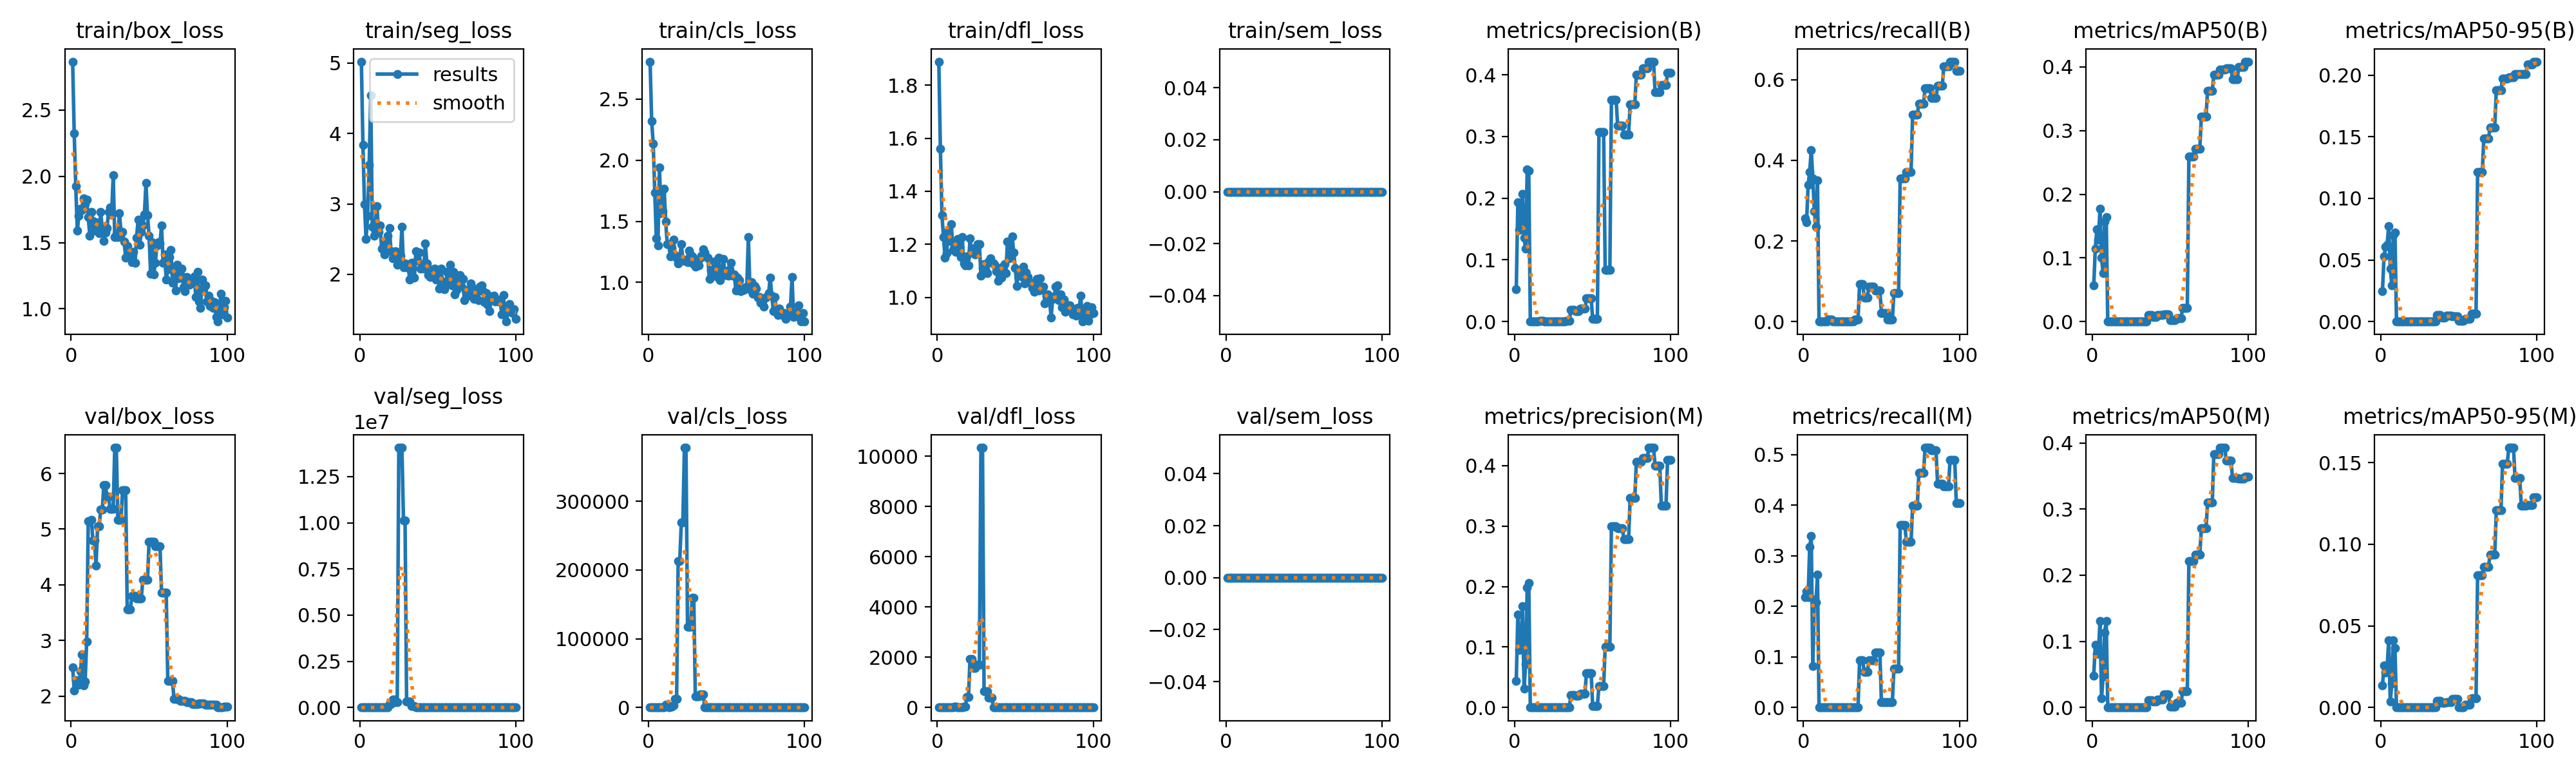
\includegraphics[width=0.92\linewidth]{assets/training/results.png}
\caption{YOLO training metrics over epochs}
\end{figure}

\begin{figure}[H]
\centering
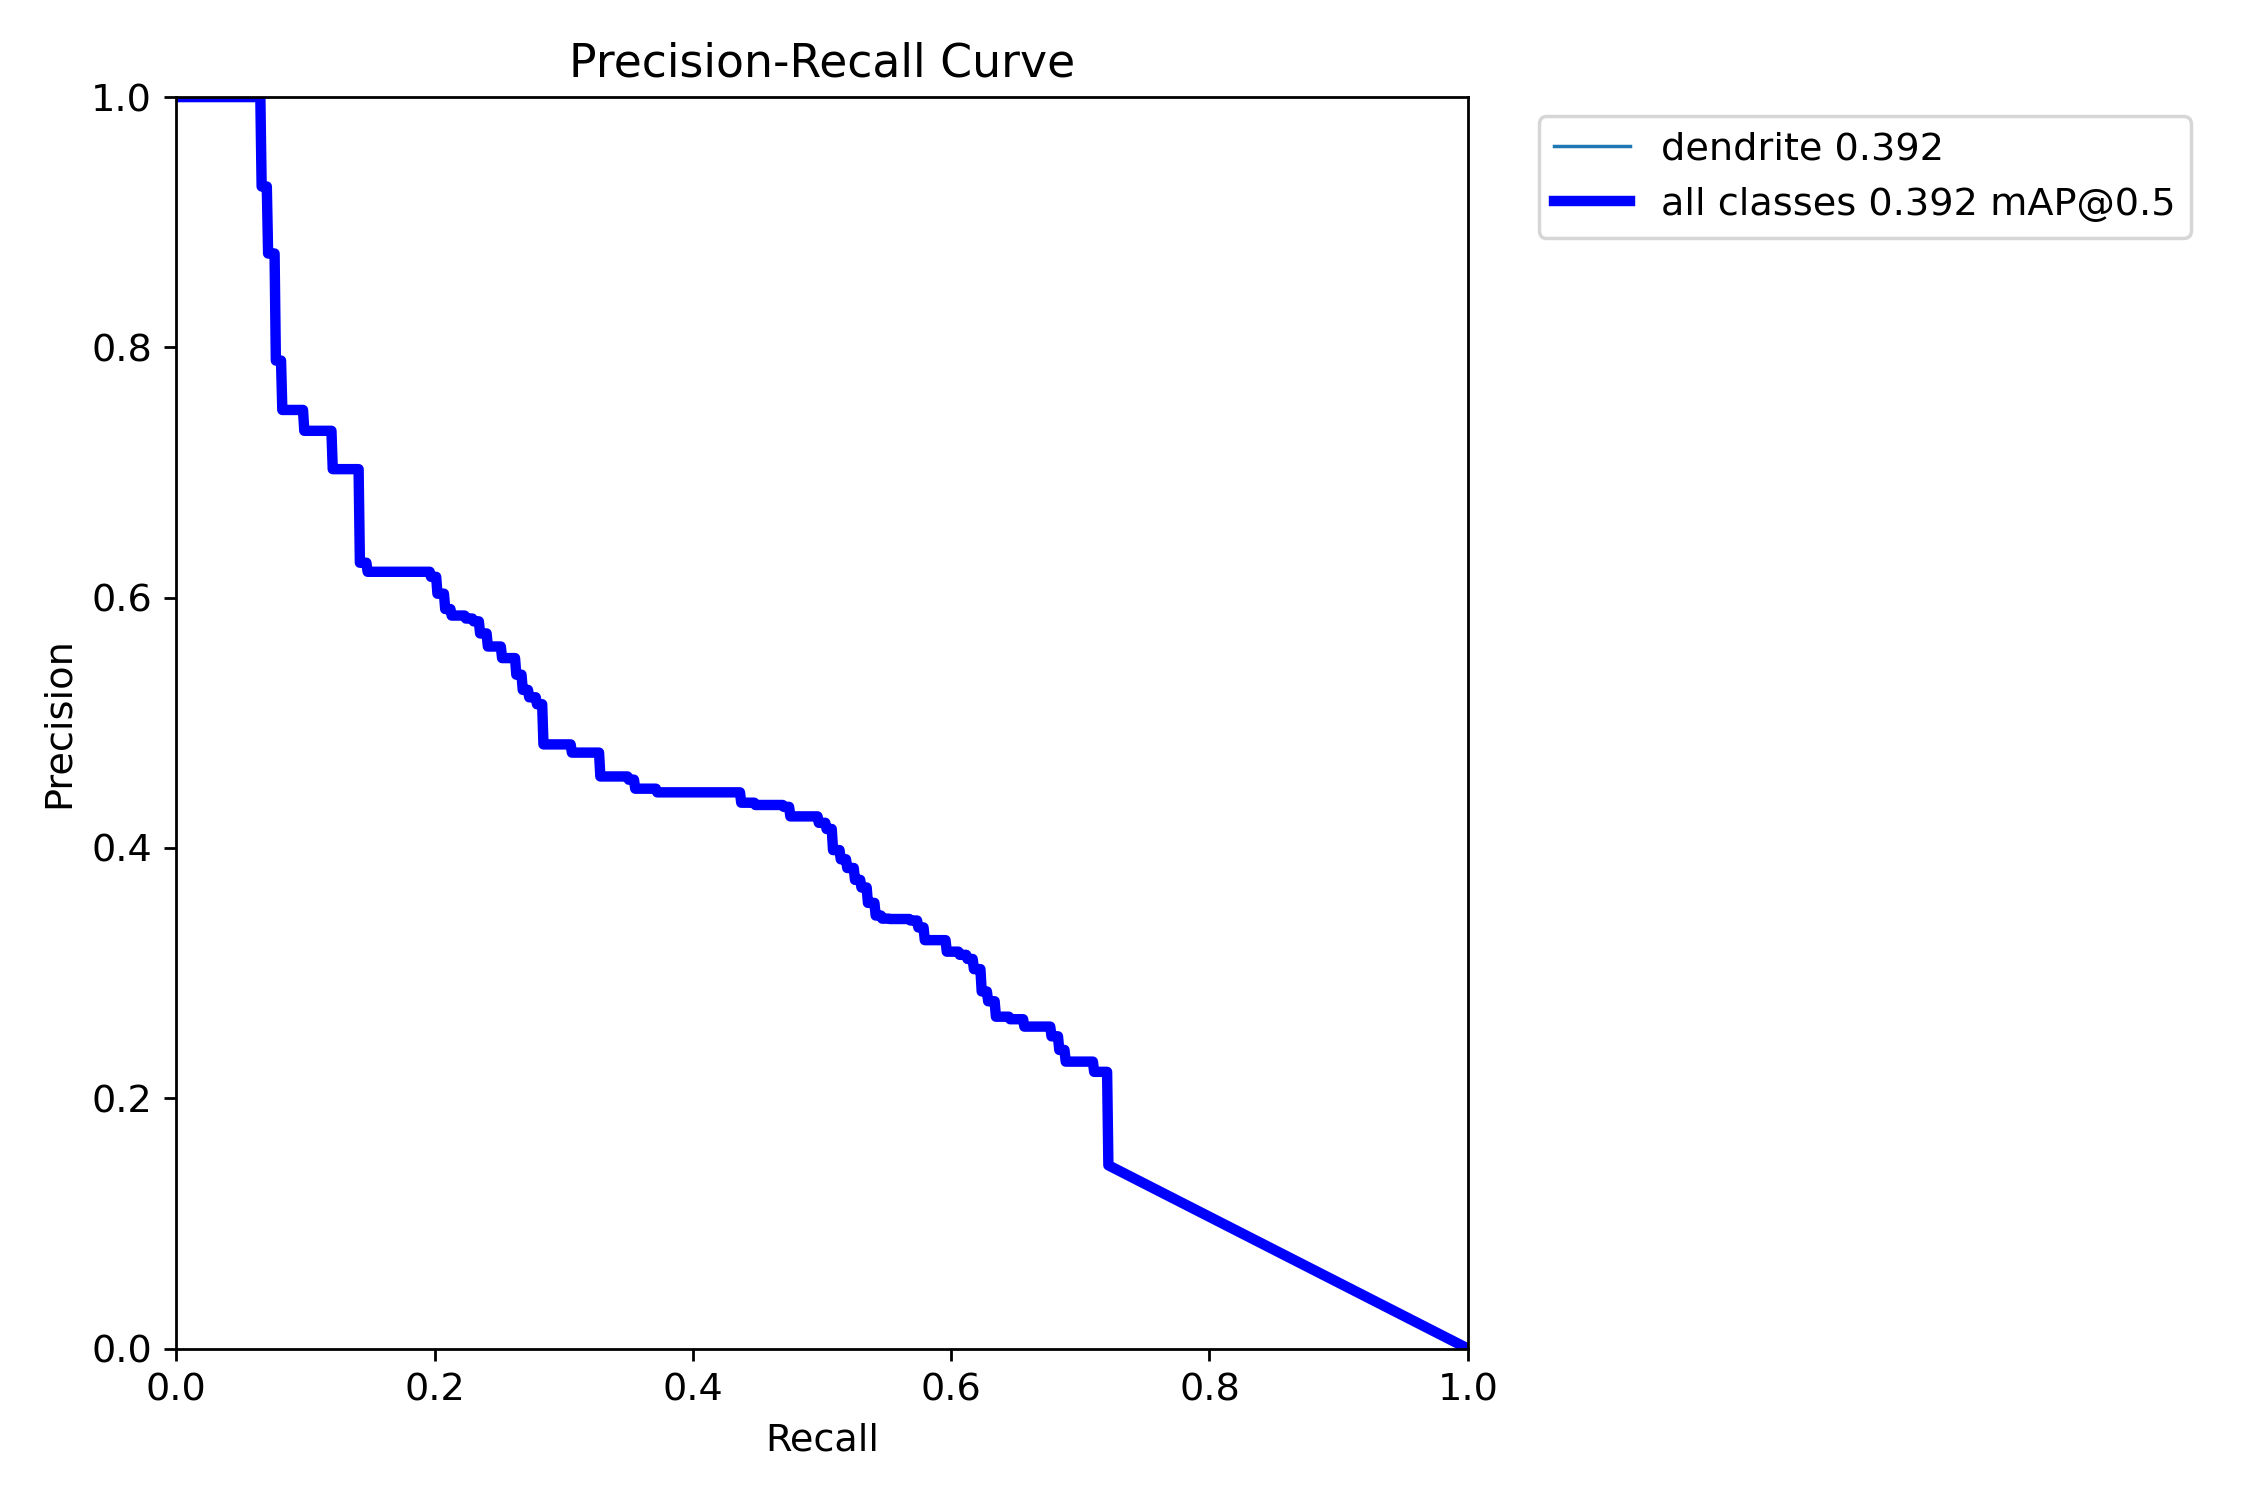
\includegraphics[width=0.92\linewidth]{assets/training/MaskPR_curve.png}
\caption{Mask precision-recall curve}
\end{figure}

\begin{figure}[H]
\centering
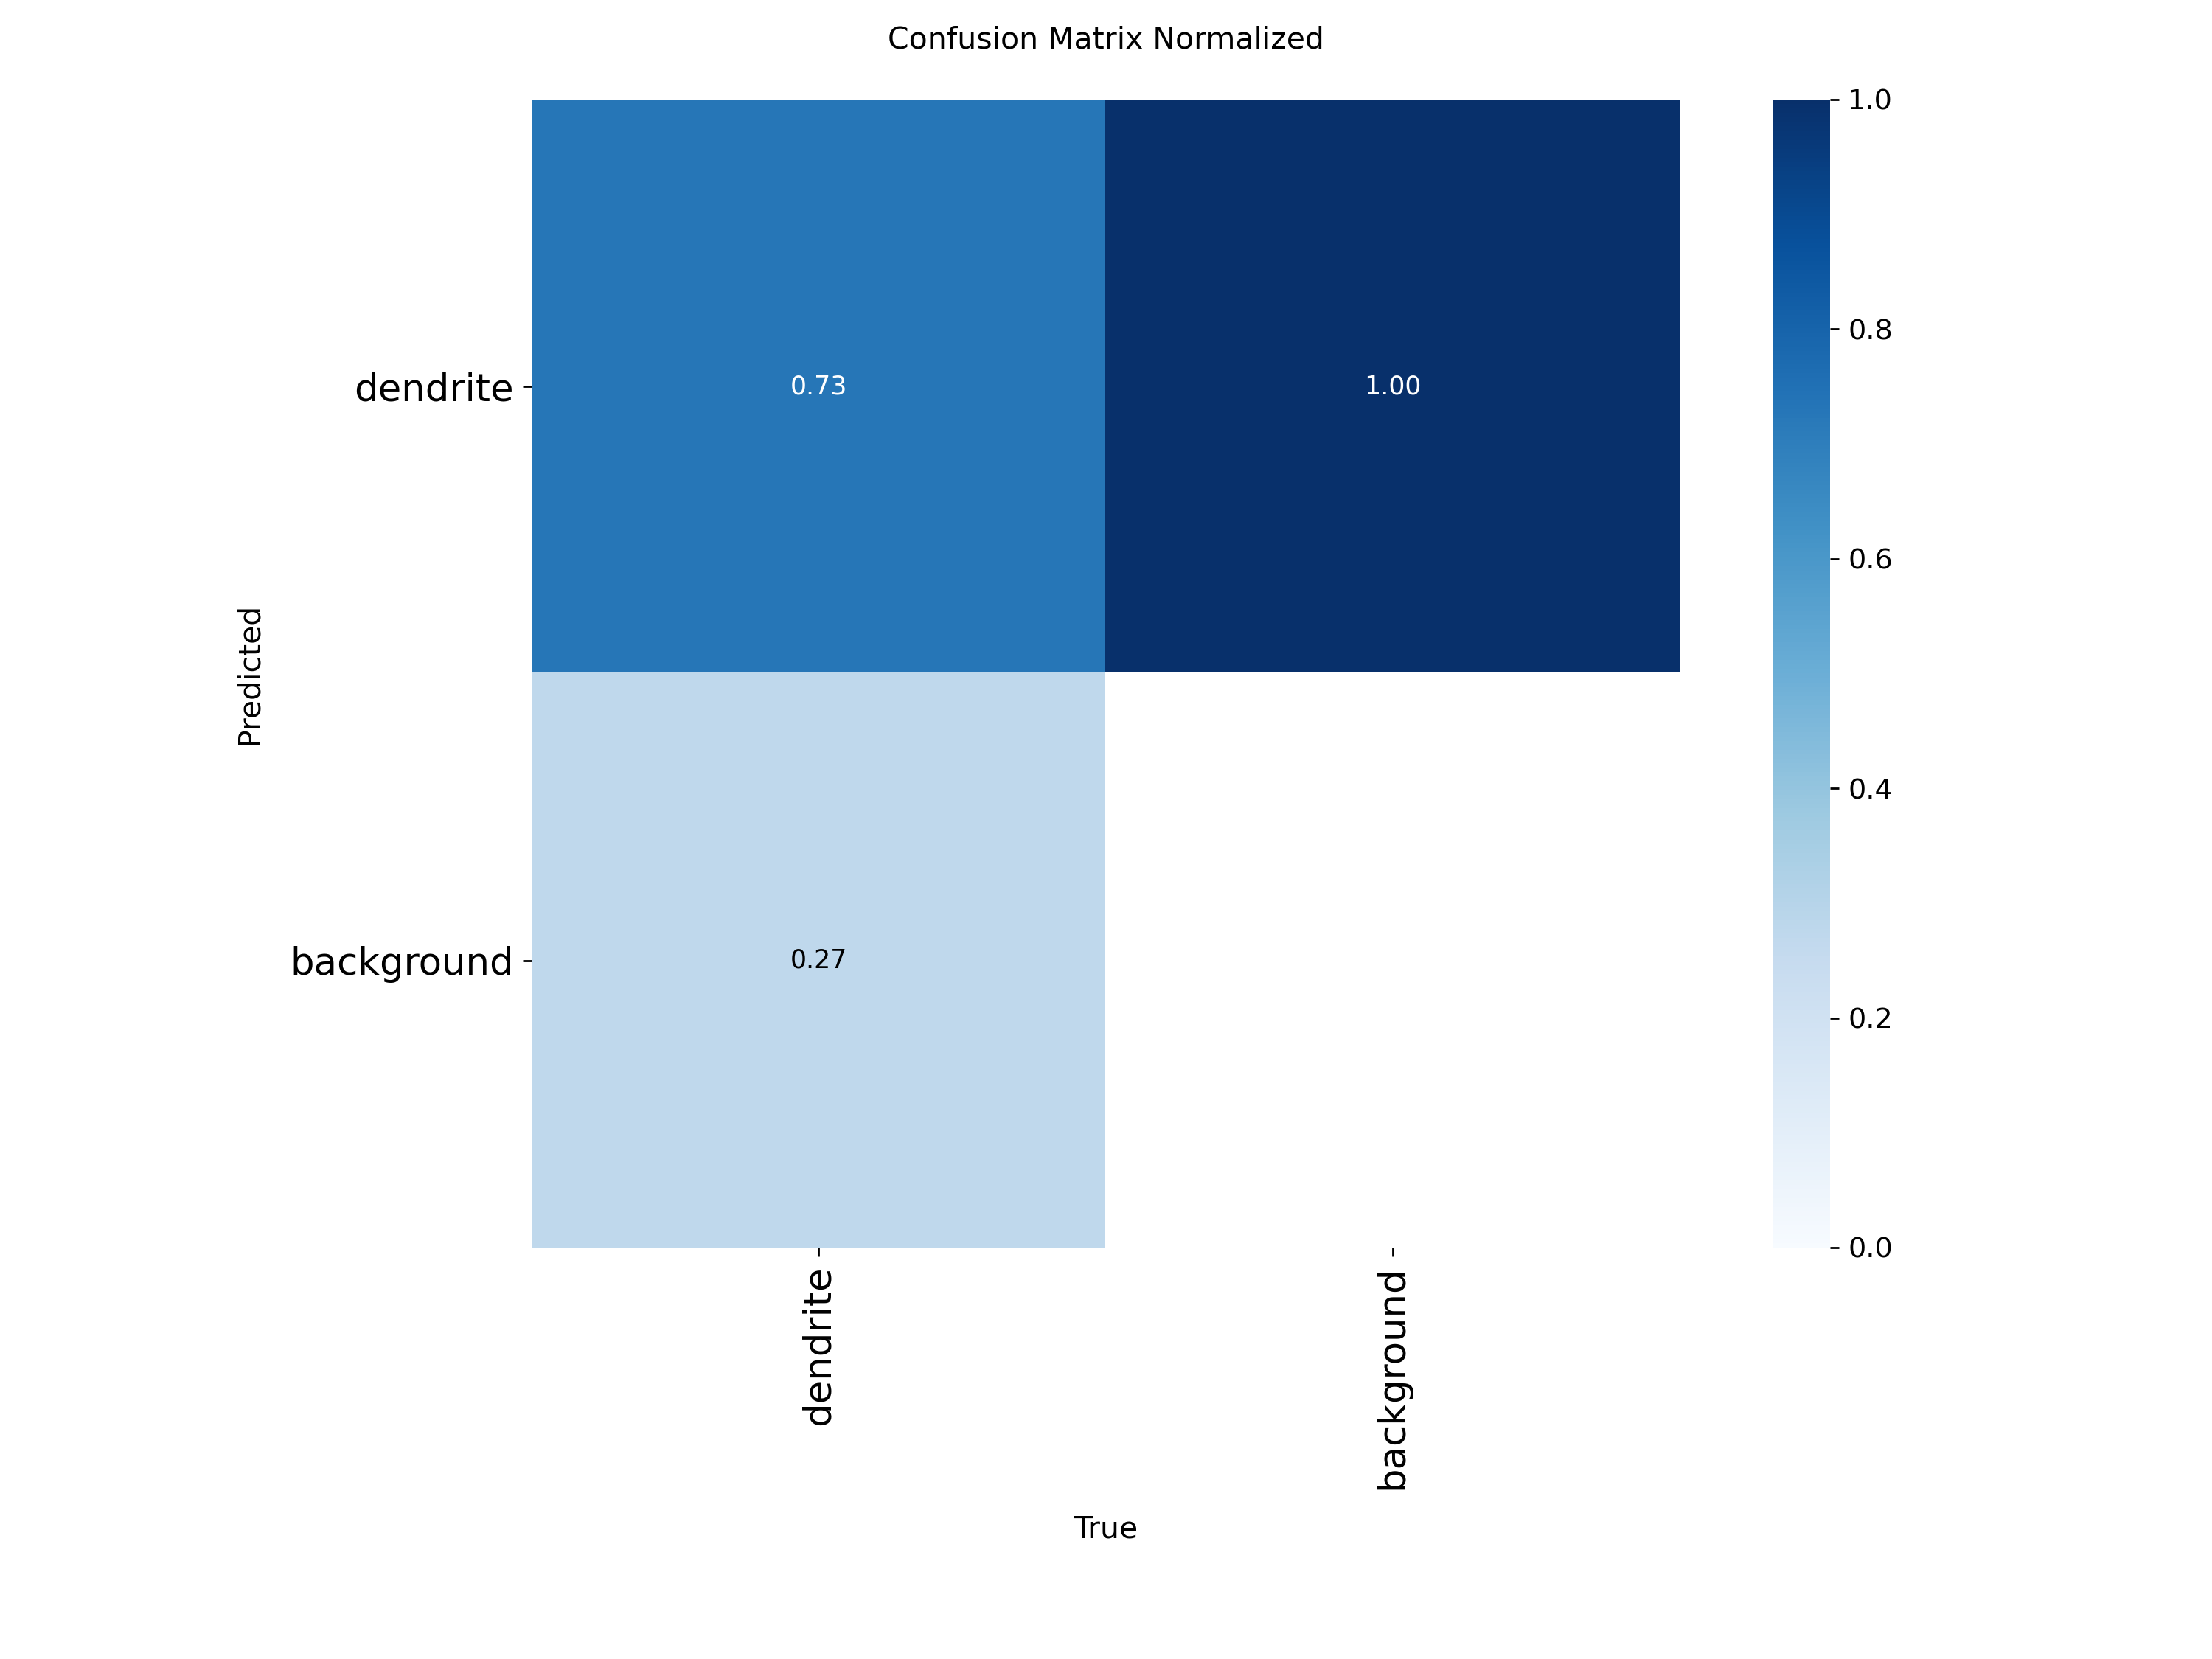
\includegraphics[width=0.92\linewidth]{assets/training/confusion_matrix_normalized.png}
\caption{Normalized confusion matrix}
\end{figure}

\section*{Conclusions}
For this dataset and preprocessing setup, the classic pipeline is the preferred primary method.
Its average Dice is 0.845 versus 0.449 for YOLO, with consistently stronger IoU and precision-recall balance across most samples.

\textbf{Which method to use in which scenario:}
\begin{enumerate}
\item \textbf{Current SEM domain with limited retraining budget:}
recommented to use \textbf{Classic pipeline} as default.
It is more stable under the current image statistics and profile split (Easy/Hard), and it produced the strongest overall segmentation quality in this report.

\item \textbf{High-throughput deployment after domain-specific retraining:}
use \textbf{YOLO} when enough representative labeled data is available and periodic retraining is feasible.
In the present run, YOLO shows useful recall behavior but suffers from domain mismatch failures and over-segmentation in several hard cases.

\item \textbf{Outlier / severe-artifact samples (e.g., 70nm\_diameter\_100nm\_pitch\_033):}
neither method is reliable enough alone; enforce \textbf{manual review / QA fallback}.
These cases should be prioritized for additional labeling and targeted parameter or model updates.
\end{enumerate}

\textbf{Recommended operating policy:}
run Classic as the baseline automatic segmenter, keep YOLO as a secondary comparator, and trigger human validation when inter-method disagreement or low-confidence behavior is detected.
This hybrid policy gives robust near-term results while preserving a path to future model-driven scaling.

\end{document}
